\documentclass[11pt,a4paper]{article}

\usepackage[margin=1.4cm]{geometry}
\usepackage[utf8]{inputenc}
\usepackage{amsmath,amssymb}
\usepackage{graphicx}
\usepackage{subcaption}
\usepackage{listings}
\usepackage{xcolor}
\usepackage{hyperref}
\usepackage{float}
\usepackage{tikz}
\usepackage{booktabs}
\usepackage{multirow}
\usepackage{enumitem}
\usepackage{caption}

\usetikzlibrary{shapes,arrows,positioning,calc,decorations.pathreplacing}

\graphicspath{{figures/}}

% Custom subsection numbering (1a, 1b, 1c instead of 1.1, 1.2, 1.3)
\renewcommand{\thesubsection}{\thesection\alph{subsection}}

% Tighter spacing
\setlength{\parskip}{0.15em}
\setlength{\parindent}{0pt}
\setlist{itemsep=1pt, topsep=2pt, parsep=1pt}
\captionsetup{font=footnotesize, skip=3pt}

% Reduce float spacing
\setlength{\textfloatsep}{6pt}
\setlength{\floatsep}{6pt}
\setlength{\intextsep}{6pt}
\setlength{\abovecaptionskip}{4pt}
\setlength{\belowcaptionskip}{2pt}

% Compact code style
\definecolor{codegreen}{rgb}{0,0.6,0}
\definecolor{backcolour}{rgb}{0.96,0.96,0.93}
\lstdefinestyle{matlab}{
    backgroundcolor=\color{backcolour},
    commentstyle=\color{codegreen},
    keywordstyle=\color{blue}\bfseries,
    basicstyle=\ttfamily\scriptsize,
    breaklines=true,
    numbers=left,
    numberstyle=\tiny\color{gray},
    numbersep=4pt,
    frame=single,
    language=Matlab,
    aboveskip=3pt,
    belowskip=3pt,
}
\lstset{style=matlab}

% TikZ styles
\tikzstyle{vertex} = [circle, draw, fill=orange!80, minimum size=0.7cm, font=\small\bfseries]
\tikzstyle{landmark} = [circle, draw, fill=green!60, minimum size=0.7cm, font=\small\bfseries]
\tikzstyle{factor} = [rectangle, fill=black, minimum size=0.2cm]

\title{\textbf{COMP0222 Coursework 01: Graph-based Optimisation and SLAM}}
\author{Harmish Zala, Muhammad Maaz, Aditya Bishnoi\\\\Department of Computer Science, University College London}
\date{\today}

\begin{document}
\maketitle

%==============================================================================
\section{Question 1: GPS-only Localisation}
%==============================================================================

\subsection{Factor Graph Structure}

This section addresses the problem of estimating a robot's trajectory using noisy odometry and GPS measurements via factor graph optimisation. The factor graph encodes all probabilistic relationships exactly through vertices (unknown states) and edges (measurement factors), unlike filtering methods such as the EKF which approximate the probability distribution.

\subsubsection*{Vertices}

The graph contains one type of vertex:

\textbf{Platform state vertex} $\mathbf{x}_k$: represents the robot's pose at timestep $k$.
\begin{equation}
    \mathbf{x}_k = \begin{bmatrix} x_k \\ y_k \\ \psi_k \end{bmatrix}
\end{equation}
where $(x_k, y_k)$ is the 2D position and $\psi_k$ is the heading angle. The update rule for applying corrections $\delta\mathbf{x}$ during optimisation is vector addition: $\mathbf{x}_k \oplus \delta\mathbf{x} = \mathbf{x}_k + \delta\mathbf{x}$, with the heading wrapped to $[-\pi, \pi]$ after each update. A new platform vertex is created at every odometry timestep ($\Delta T = 0.2$\,s), so the graph grows linearly with time.

\subsubsection*{Edges (Factors)}

There are three types of edges:

\begin{enumerate}
\item \textbf{Initial prior edge} (unary, connects to $\mathbf{x}_0$ only). This anchors the initial pose and establishes the global reference frame. Without it, the entire graph could shift freely since all other constraints are relative. The measurement is $\mathbf{z}_0 = [0, 0, 0]^T$, the error is $\mathbf{e}_{\text{prior}} = \mathbf{x}_0 - \mathbf{z}_0$, and the information matrix is $\boldsymbol{\Omega}_0 = \mathbf{P}_0^{-1}$. In our setup $\mathbf{P}_0 = \mathbf{0}$, making this prior infinitely strong.

\item \textbf{Platform prediction edge} (binary, connects $\mathbf{x}_k$ to $\mathbf{x}_{k+1}$). This encodes the odometry-based motion model. At each timestep, wheel encoders provide body-frame velocity measurements $\mathbf{u}_{k+1} = [v_x, v_y, \dot{\psi}]^T$. The process model predicts:
\begin{equation}
    \mathbf{x}_{k+1} = \mathbf{x}_k + \mathbf{M}(\psi_k) \, \mathbf{u}_{k+1}
\end{equation}
where $\mathbf{M}(\psi_k)$ is the scaled rotation matrix transforming body-frame velocities to world-frame displacements:
\begin{equation}
    \mathbf{M}(\psi_k) = \Delta T \begin{bmatrix} \cos\psi_k & -\sin\psi_k & 0 \\ \sin\psi_k & \cos\psi_k & 0 \\ 0 & 0 & 1 \end{bmatrix}
    \label{eq:M_matrix}
\end{equation}
The process noise is $\mathbf{w} \sim \mathcal{N}(\mathbf{0}, \mathbf{Q})$ with $\sigma_Q = [0.2, 0.1, 1.0]$ (forward, lateral, yaw rate). The information matrix is $\boldsymbol{\Omega}_Q = \mathbf{Q}^{-1}$. One prediction edge is added per timestep, linking consecutive poses.

\item \textbf{GPS measurement edge} (unary, connects to a single $\mathbf{x}_k$). The GPS sensor directly measures position $(x, y)$ with additive Gaussian noise:
\begin{equation}
    \mathbf{z}_k^G = \begin{bmatrix} x_k \\ y_k \end{bmatrix} + \mathbf{w}_k^G, \quad \mathbf{w}_k^G \sim \mathcal{N}(\mathbf{0}, \mathbf{R}^G)
\end{equation}
where $\sigma_R = 1$\,m. The error is $\mathbf{e}_{\text{GPS}} = \mathbf{z}_k^G - [x_k,\; y_k]^T$. This 2D edge constrains position only, not heading. GPS measurements arrive every 2\,s, so one GPS edge is added every 10 odometry steps.
\end{enumerate}

\subsubsection*{Factor Graph Diagram}

Figure~\ref{fig:q1a_factor_graph} shows the structure. At each timestep, a new platform vertex and prediction edge are added. Every 10 timesteps, a GPS factor is also attached.

\begin{figure}[H]
\centering
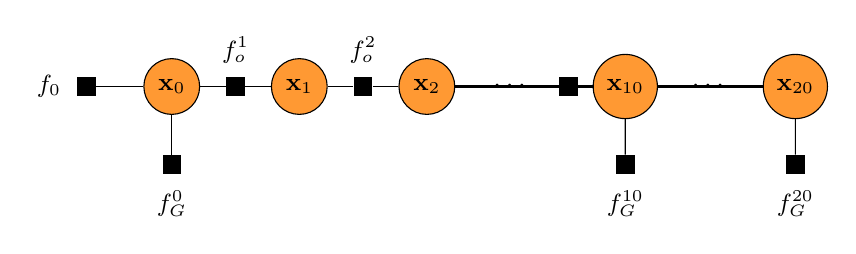
\begin{tikzpicture}[scale=0.9]
    \node[vertex] (x0) at (0,0) {$\mathbf{x}_0$};
    \node[factor] (f0) at (-1.2,0) {};
    \draw (f0) -- (x0);
    \node[left=0.08cm of f0] {\small $f_0$};
    \node[vertex] (x1) at (1.8,0) {$\mathbf{x}_1$};
    \node[factor] (f1) at (0.9,0) {};
    \draw (x0) -- (f1) -- (x1);
    \node[above=0.05cm of f1] {\small $f_o^1$};
    \node[vertex] (x2) at (3.6,0) {$\mathbf{x}_2$};
    \node[factor] (f2) at (2.7,0) {};
    \draw (x1) -- (f2) -- (x2);
    \node[above=0.05cm of f2] {\small $f_o^2$};
    \node at (4.8,0) {$\cdots$};
    \node[vertex] (x10) at (6.4,0) {$\mathbf{x}_{10}$};
    \node[factor] (f10) at (5.6,0) {};
    \draw[thick] (x2) -- (4.8,0);
    \draw[thick] (4.8,0) -- (f10) -- (x10);
    \node at (7.6,0) {$\cdots$};
    \node[vertex] (x20) at (8.8,0) {$\mathbf{x}_{20}$};
    \draw[thick] (x10) -- (7.6,0);
    \draw[thick] (7.6,0) -- (x20);
    \node[factor] (g0) at (0,-1.1) {};
    \draw (g0) -- (x0);
    \node[below=0.08cm of g0] {\small $f_G^0$};
    \node[factor] (g10) at (6.4,-1.1) {};
    \draw (g10) -- (x10);
    \node[below=0.08cm of g10] {\small $f_G^{10}$};
    \node[factor] (g20) at (8.8,-1.1) {};
    \draw (g20) -- (x20);
    \node[below=0.08cm of g20] {\small $f_G^{20}$};
\end{tikzpicture}
\caption{GPS-only localisation factor graph. Orange circles are platform state vertices. Black squares are factors. Prediction edges link consecutive poses; GPS edges attach to individual poses.}
\label{fig:q1a_factor_graph}
\end{figure}

\subsubsection*{Optimisation Objective}

The optimiser finds $\mathbf{x}_{0:K}^*$ minimising the total weighted squared error:
\begin{equation}
    \mathbf{x}^* = \arg\min_{\mathbf{x}_{0:K}} \sum_{i} \mathbf{e}_i^T \, \boldsymbol{\Omega}_i \, \mathbf{e}_i
    \label{eq:cost_function}
\end{equation}
where $i$ ranges over all edges. The information matrix $\boldsymbol{\Omega}_i$ weights each term so that lower-noise measurements pull the solution more strongly. This is solved iteratively using Gauss-Newton or Levenberg-Marquardt: at each iteration, the system linearises all error functions, builds the sparse Hessian $\mathbf{H} = \sum_i \mathbf{J}_i^T \boldsymbol{\Omega}_i \mathbf{J}_i$, and solves a linear system to compute the update.

\subsection{PlatformPredictionEdge Implementation}

The \texttt{PlatformPredictionEdge} is a binary edge connecting consecutive platform vertices $\mathbf{x}_k$ and $\mathbf{x}_{k+1}$. It implements three methods:

\subsubsection*{Initial Estimate}

When a new vertex $\mathbf{x}_{k+1}$ is created, its initial estimate is computed by forward-propagating the process model from $\mathbf{x}_k$:

\begin{lstlisting}
function initialEstimate(obj)
    x_k = obj.edgeVertices{1}.estimate();
    psi_k = x_k(3);
    u = obj.z;   % odometry: [vx; vy; omega]
    c = cos(psi_k);  s = sin(psi_k);
    M = obj.dT * [c, -s, 0; s, c, 0; 0, 0, 1];
    x_kp1 = x_k + M * u;
    x_kp1(3) = g2o.stuff.normalize_theta(x_kp1(3));
    obj.edgeVertices{2}.setEstimate(x_kp1);
end
\end{lstlisting}

This implements $\mathbf{x}_{k+1} = \mathbf{x}_k + \mathbf{M}(\psi_k)\,\mathbf{u}$ with heading wrapped to $[-\pi, \pi]$.

\subsubsection*{Error Computation}

The error measures how well the two connected vertices agree with the odometry. It is computed in the \emph{body frame} so $\boldsymbol{\Omega}_Q = \mathbf{Q}^{-1}$ can be used directly (since odometry noise is defined in the body frame):
\begin{equation}
    \mathbf{e} = \mathbf{M}^{-1}(\psi_k) \, (\mathbf{x}_{k+1} - \mathbf{x}_k) - \mathbf{u}
    \label{eq:pred_error}
\end{equation}
where $\mathbf{M}^{-1}$ is straightforward since the rotation matrix is orthogonal:
\begin{equation}
    \mathbf{M}^{-1}(\psi_k) = \frac{1}{\Delta T} \begin{bmatrix} \cos\psi_k & \sin\psi_k & 0 \\ -\sin\psi_k & \cos\psi_k & 0 \\ 0 & 0 & 1 \end{bmatrix}
    \label{eq:M_inverse}
\end{equation}
The idea is to take the world-frame displacement $(\mathbf{x}_{k+1} - \mathbf{x}_k)$, rotate it back to the body frame via $\mathbf{M}^{-1}$, and compare with the odometry $\mathbf{u}$. If the edge perfectly explains the data, the error is zero.

\begin{lstlisting}
function computeError(obj)
    x_k   = obj.edgeVertices{1}.estimate();
    x_kp1 = obj.edgeVertices{2}.estimate();
    psi_k = x_k(3);
    c = cos(psi_k);  s = sin(psi_k);
    invM = (1/obj.dT) * [c, s, 0; -s, c, 0; 0, 0, 1];
    obj.errorZ = invM * (x_kp1 - x_k) - obj.z;
    obj.errorZ(3) = g2o.stuff.normalize_theta(obj.errorZ(3));
end
\end{lstlisting}

\subsubsection*{Jacobian Computation}

The optimiser needs $\mathbf{J}_1 = \frac{\partial \mathbf{e}}{\partial \mathbf{x}_k}$ and $\mathbf{J}_2 = \frac{\partial \mathbf{e}}{\partial \mathbf{x}_{k+1}}$ to build the Hessian. These are derived analytically for accuracy and speed.

Let $\boldsymbol{\delta} = \mathbf{x}_{k+1} - \mathbf{x}_k = [\delta_x, \delta_y, \delta_\psi]^T$. The error from Eq.~\eqref{eq:pred_error} is:
\begin{equation}
    \mathbf{e} = \frac{1}{\Delta T}
    \begin{bmatrix}
        \cos\psi\,\delta_x + \sin\psi\,\delta_y \\
        -\sin\psi\,\delta_x + \cos\psi\,\delta_y \\
        \delta_\psi
    \end{bmatrix}
    - \mathbf{u}
\end{equation}

\textbf{Jacobian w.r.t.\ $\mathbf{x}_{k+1}$:} Since $\boldsymbol{\delta}$ depends linearly on $\mathbf{x}_{k+1}$:
\begin{equation}
    \mathbf{J}_2 = \frac{\partial \mathbf{e}}{\partial \mathbf{x}_{k+1}} = \mathbf{M}^{-1} = \frac{1}{\Delta T}
    \begin{bmatrix}
        \cos\psi & \sin\psi & 0 \\
        -\sin\psi & \cos\psi & 0 \\
        0 & 0 & 1
    \end{bmatrix}
\end{equation}

\textbf{Jacobian w.r.t.\ $\mathbf{x}_k$:} More involved because $\mathbf{x}_k$ appears in both $\boldsymbol{\delta}$ and $\mathbf{M}^{-1}$ (through $\psi_k$). Using the product rule:
\begin{equation}
    \mathbf{J}_1 = \frac{\partial \mathbf{e}}{\partial \mathbf{x}_k} = \frac{1}{\Delta T}
    \begin{bmatrix}
        -\cos\psi & -\sin\psi & -\sin\psi\,\delta_x + \cos\psi\,\delta_y \\
        \sin\psi & -\cos\psi & -\cos\psi\,\delta_x - \sin\psi\,\delta_y \\
        0 & 0 & -1
    \end{bmatrix}
\end{equation}
The first two columns are $-\mathbf{M}^{-1}$ (from $\frac{\partial \boldsymbol{\delta}}{\partial x_k} = -\mathbf{I}$). The third column has an extra term because changing $\psi_k$ also changes the rotation in $\mathbf{M}^{-1}$.

\begin{lstlisting}
function linearizeOplus(obj)
    x_k   = obj.edgeVertices{1}.estimate();
    x_kp1 = obj.edgeVertices{2}.estimate();
    psi_k = x_k(3);
    c = cos(psi_k);  s = sin(psi_k);
    delta = x_kp1 - x_k;
    dx = delta(1);  dy = delta(2);
    invM = (1/obj.dT) * [c, s, 0; -s, c, 0; 0, 0, 1];
    dInvMdelta_dpsi = (1/obj.dT) * [-s*dx + c*dy; -c*dx - s*dy; 0];
    obj.J{1} = -invM;
    obj.J{1}(:,3) = obj.J{1}(:,3) + dInvMdelta_dpsi;
    obj.J{2} = invM;
end
\end{lstlisting}

\subsubsection*{Results}

Running \texttt{cw1.q1\_b} produces the trajectory and error plots in Figure~\ref{fig:q1b_results}.

\begin{figure}[H]
\centering
\begin{subfigure}[b]{0.46\textwidth}
    \includegraphics[width=\textwidth]{q1b_02_Q1b_Trajectory_Comparison.png}
    \caption{True vs estimated trajectory.}
\end{subfigure}
\hfill
\begin{subfigure}[b]{0.46\textwidth}
    \includegraphics[width=\textwidth]{q1b_01_Q1b_State_Estimation_Errors.png}
    \caption{State errors with $\pm 2\sigma$ bounds.}
\end{subfigure}
\caption{Q1b: Trajectory comparison and state estimation errors.}
\label{fig:q1b_results}
\end{figure}

\begin{table}[H]
\centering\small
\begin{tabular}{lccc}
\toprule
 & $x$ & $y$ & $\psi$ \\
\midrule
RMSE & 0.356\,m & 0.482\,m & 0.024\,rad (1.35\textdegree) \\
Final $2\sigma$ bound & 0.860\,m & 0.612\,m & 0.049\,rad \\
\% within $2\sigma$ & 100.0\% & 71.7\% & 96.2\% \\
\bottomrule
\end{tabular}
\caption{Q1b estimation performance summary.}
\label{tab:q1b_results}
\end{table}

\textbf{Analysis:} The estimated trajectory (blue dashed) closely tracks the ground truth (green), showing that the combination of odometry and GPS corrections successfully recovers the robot's path. The small deviations are expected given $\sigma = 1$\,m GPS noise.

\begin{itemize}
    \item \textbf{$x$ state (100\% within bounds):} The $x$ error stays well within the $2\sigma$ band throughout. The bounds settle to $\pm 0.86$\,m, matching the GPS noise level. No visible drift, confirming GPS corrections prevent odometry drift accumulation.

    \item \textbf{$y$ state (71.7\% within bounds):} Notably lower than the expected 95.4\%. The $y$ error temporarily exceeds bounds during parts of the trajectory. This occurs because the covariance bounds from the graph's Hessian assume perfect linearisation, but the process model's nonlinear dependence on heading ($\cos\psi$, $\sin\psi$) makes linearisation less accurate during turns. The $y$ direction is more affected because the trajectory involves more lateral motion components where heading uncertainty maps into $y$ position uncertainty. This is a known limitation of linearised optimisation: the covariance can be too optimistic when nonlinearity is significant.

    \item \textbf{$\psi$ state (96.2\% within bounds):} Close to the expected 95.4\%, showing well-calibrated heading estimation. The heading RMSE is 0.024\,rad $\approx$ 1.35\textdegree. Even though GPS doesn't directly measure heading, it is indirectly constrained by the sequence of position corrections: consecutive GPS fixes that show the robot has moved in a certain direction constrain what the heading must have been.
\end{itemize}

The RMSE values (0.36\,m in $x$, 0.48\,m in $y$) are sub-meter, reasonable given 1\,m GPS noise. The heading RMSE of 1.35\textdegree{} is small because the odometry provides strong heading information ($\sigma_\omega = 1$\,rad/s scaled by $\Delta T = 0.2$\,s gives $\sigma_{\Delta\psi} = 0.2$\,rad per step, but many consecutive steps constrain the cumulative heading well).

\subsection{Graph Optimisation Analysis}

Running \texttt{cw1.q1\_c} optimises the graph at every timestep, letting us observe how $\chi^2$ cost and optimisation time evolve as the graph grows.

\begin{figure}[H]
\centering
\includegraphics[width=0.58\textwidth]{q1c_01_Q1c_Chi2_and_Optimisation_Time.png}
\caption{Q1c: $\chi^2$ cost and optimisation duration over 814 steps.}
\label{fig:q1c_chi2}
\end{figure}

\begin{table}[H]
\centering\small
\begin{tabular}{ll|ll}
\toprule
Total optimisation steps & 814 & Mean optimisation time & 0.0033\,s \\
$\chi^2$ range & $[0.00,\; 46.82]$ & Max optimisation time & 0.073\,s \\
$\chi^2$ growth rate & $0.069$/step & Timing growth rate & $7 \times 10^{-6}$\,s/step \\
\bottomrule
\end{tabular}
\caption{Q1c optimisation statistics.}
\label{tab:q1c_stats}
\end{table}

\subsubsection*{Analysis of the $\chi^2$ plot (top)}

The $\chi^2$ value increases over time following a clear \textbf{staircase pattern}, with each step corresponding to a new GPS measurement. Between GPS events (every 2\,s = 10 timesteps), $\chi^2$ stays flat. Prediction edges, initialised via forward propagation through \texttt{initialEstimate()}, exhibit near-zero residuals, contributing negligibly to the cost. Conversely, GPS measurements exhibit non-zero discrepancies due to sensor noise, and the optimiser cannot fully eliminate these residuals without violating odometry constraints. Each GPS observation thus introduces an irreducible residual, manifesting as discrete upward steps.

The linear fit gives $\chi^2 \approx 0.069 \times \text{step}$, so each GPS measurement adds roughly $0.69$ to the total cost. For a 2D measurement with $\sigma = 1$\,m, we'd expect $\mathbb{E}[\chi^2_2] = 2$ on average; the lower observed value occurs because the optimiser adjusts the trajectory to partially absorb GPS residuals. The steady linear growth confirms the system is working correctly.

\subsubsection*{Analysis of the optimisation time plot (bottom)}

The optimisation time shows a general upward trend with spikes, with growth rate $7 \times 10^{-6}$\,s per step. Each iteration requires assembly and factorisation of $\mathbf{H} = \sum_i \mathbf{J}_i^T \boldsymbol{\Omega}_i \mathbf{J}_i$, with dimensionality $3K \times 3K$. The chain topology induces a banded Hessian, yielding $O(K)$ factorisation complexity and explaining the approximately linear timing growth. The spikes occur when GPS measurements arrive, as the new residuals may cause Levenberg-Marquardt to need more iterations to converge.

\subsubsection*{Root cause}

Both trends share the same underlying cause: \textbf{the graph grows without bound}. Every timestep adds a new vertex and edge with nothing removed, so more error terms lead to higher total $\chi^2$ and a larger Hessian means more computation per step. This motivates the graph management strategies explored in Question~3.

\subsubsection*{Estimation quality}

Despite running the optimiser at every step, the estimation quality (Table~\ref{tab:q1c_est}) is similar to Q1b:

\begin{table}[H]
\centering\small
\begin{tabular}{lccc}
\toprule
 & $x$ & $y$ & $\psi$ \\
\midrule
RMSE & 0.295\,m & 0.250\,m & 0.019\,rad (1.08\textdegree) \\
\% within $2\sigma$ & 91.1\% & 99.5\% & 98.5\% \\
\bottomrule
\end{tabular}
\caption{Q1c estimation performance.}
\label{tab:q1c_est}
\end{table}

The RMSE values are slightly better than Q1b (which optimised less frequently). The $2\sigma$ consistency improved significantly, particularly for $y$ (from 71.7\% to 99.5\%), because optimising at every step gives the graph more chances to adjust the trajectory, reducing linearisation errors (each update is a small perturbation from the current estimate).

\begin{figure}[H]
\centering
\begin{subfigure}[b]{0.46\textwidth}
    \includegraphics[width=\textwidth]{q1c_03_Q1c_Trajectory_Comparison.png}
    \caption{True vs estimated trajectory.}
\end{subfigure}
\hfill
\begin{subfigure}[b]{0.46\textwidth}
    \includegraphics[width=\textwidth]{q1c_02_Q1c_State_Estimation_Errors.png}
    \caption{State errors with $\pm 2\sigma$ bounds.}
\end{subfigure}
\caption{Q1c: Trajectory and state errors. Compared to Q1b, $y$ consistency improved from 71.7\% to 99.5\%.}
\label{fig:q1c_results}
\end{figure}

%==============================================================================
\section{Question 2: Full SLAM Implementation}
%==============================================================================

\subsection{Factor Graph Structure for Full SLAM}

Full SLAM extends the GPS-only setup by adding \emph{landmarks} to the state and \emph{range-bearing observations} as new constraints. The robot now estimates both its own trajectory and landmark positions, solving the coupled localisation and mapping problem together.

\subsubsection*{New Vertex Type}

\textbf{Landmark state vertex} $\mathbf{m}_i$: represents the 2D position of the $i$-th landmark in the world frame, $\mathbf{m}_i = [m_x,\; m_y]^T$. The dimension is 2 and the update rule is standard addition: $\mathbf{m}_i \oplus \delta\mathbf{m} = \mathbf{m}_i + \delta\mathbf{m}$. Unlike platform vertices (which grow linearly with time), landmark vertices are created once per landmark and persist for the entire run.

\subsubsection*{New Edge Type}

\textbf{Landmark range-bearing edge} (binary, connects $\mathbf{x}_k$ to $\mathbf{m}_i$). When the robot observes landmark $i$ from pose $k$, it measures range $r$ and bearing $\beta$:
\begin{equation}
    \mathbf{z}^L = \begin{bmatrix} r \\ \beta \end{bmatrix} = \mathbf{h}(\mathbf{x}_k, \mathbf{m}_i) + \mathbf{w}^L
\end{equation}
where:
\begin{equation}
    r = \sqrt{(m_x - x_k)^2 + (m_y - y_k)^2}, \qquad
    \beta = \mathrm{atan2}(m_y - y_k,\; m_x - x_k) - \psi_k
    \label{eq:obs_model}
\end{equation}
The noise is $\mathbf{w}^L \sim \mathcal{N}(\mathbf{0}, \mathbf{R}^L)$ with $\sigma_r = 0.1$\,m, $\sigma_\beta = 1$\,rad in Q2b, or $\sigma_r = 1$\,m, $\sigma_\beta = 0.1$\,rad in Q2c. Each observation edge connects a platform vertex to a landmark vertex, so improving one landmark estimate can improve pose estimates and vice versa. Landmarks seen from multiple poses act as shared constraints, tying distant parts of the trajectory together.

\subsubsection*{Factor Graph Diagram}

\begin{figure}[H]
\centering
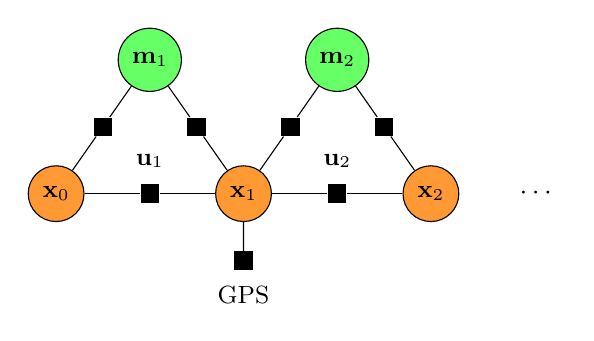
\begin{tikzpicture}[scale=0.85]
    \node[landmark] (m1) at (1.4,2) {$\mathbf{m}_1$};
    \node[landmark] (m2) at (4.2,2) {$\mathbf{m}_2$};
    \node[vertex] (x0) at (0,0) {$\mathbf{x}_0$};
    \node[vertex] (x1) at (2.8,0) {$\mathbf{x}_1$};
    \node[vertex] (x2) at (5.6,0) {$\mathbf{x}_2$};
    \node at (7.2,0) {$\cdots$};
    \node[factor] (f01) at (1.4,0) {};
    \node[factor] (f12) at (4.2,0) {};
    \draw (x0) -- (f01) -- (x1) -- (f12) -- (x2);
    \node[above=0.08cm of f01] {\small $\mathbf{u}_1$};
    \node[above=0.08cm of f12] {\small $\mathbf{u}_2$};
    \node[factor] (o1) at (0.7,1) {};
    \node[factor] (o2) at (2.1,1) {};
    \node[factor] (o3) at (3.5,1) {};
    \node[factor] (o4) at (4.9,1) {};
    \draw (x0) -- (o1) -- (m1);
    \draw (x1) -- (o2) -- (m1);
    \draw (x1) -- (o3) -- (m2);
    \draw (x2) -- (o4) -- (m2);
    \node[factor] (gps) at (2.8,-1) {};
    \draw (gps) -- (x1);
    \node[below=0.08cm of gps] {\small GPS};
\end{tikzpicture}
\caption{Full SLAM factor graph. Green: landmark vertices. Orange: platform vertices. Observation edges link poses to landmarks; prediction edges link consecutive poses.}
\label{fig:q2a_factor_graph}
\end{figure}

The key structural difference from Q1 is that the graph is no longer a simple chain. Landmark vertices connect to multiple platform vertices across time, creating cross-links that allow the optimiser to correct past pose estimates when a landmark is re-observed (the ``loop closure'' effect).

\subsubsection*{Optimisation Objective}

The full SLAM cost function extends Eq.~\eqref{eq:cost_function} to include both poses and landmarks:
\begin{equation}
    \{\mathbf{x}^*, \mathbf{m}^*\} = \arg\min_{\mathbf{x}_{0:K}, \mathbf{m}_{1:L}} \;
    \underbrace{\sum_{k} \mathbf{e}_{\text{pred},k}^T \boldsymbol{\Omega}_Q \, \mathbf{e}_{\text{pred},k}}_{\text{odometry}}
    + \underbrace{\sum_{k,i} \mathbf{e}_{\text{obs},k,i}^T \boldsymbol{\Omega}_R \, \mathbf{e}_{\text{obs},k,i}}_{\text{landmark observations}}
    + \underbrace{\sum_{k} \mathbf{e}_{\text{GPS},k}^T \boldsymbol{\Omega}_G \, \mathbf{e}_{\text{GPS},k}}_{\text{GPS (if present)}}
\end{equation}
The Hessian $\mathbf{H}$ now has pose-pose, pose-landmark, and landmark-landmark blocks.

\subsection{LandmarkRangeBearingEdge Implementation}

The \texttt{LandmarkRangeBearingEdge} is a binary edge connecting platform vertex $\mathbf{x}_k$ (vertex 1) and landmark vertex $\mathbf{m}_i$ (vertex 2).

\subsubsection*{Initial Estimate}

When a landmark is first observed, its position is initialised via the inverse observation model. The world-frame angle to the landmark is $\phi = \psi + \beta$, so:
\begin{equation}
    \mathbf{m} = \begin{bmatrix} x \\ y \end{bmatrix} + r \begin{bmatrix} \cos\phi \\ \sin\phi \end{bmatrix}
    \label{eq:inverse_obs}
\end{equation}

\begin{lstlisting}
function initialEstimate(obj)
    x_p = obj.edgeVertices{1}.estimate();  % [x; y; psi]
    r    = obj.z(1);    % range
    beta = obj.z(2);    % bearing (body frame)
    phi = x_p(3) + beta;   % world-frame angle to landmark
    m_x = x_p(1) + r * cos(phi);
    m_y = x_p(2) + r * sin(phi);
    obj.edgeVertices{2}.setEstimate([m_x; m_y]);
end
\end{lstlisting}

If the measurements are noisy, this initial guess will be imprecise, but the optimiser refines it as more observations come in.

\subsubsection*{Error Computation}

The error is $\mathbf{e} = \mathbf{z} - \mathbf{h}(\mathbf{x}_k, \mathbf{m}_i)$ where $\mathbf{h}$ is from Eq.~\eqref{eq:obs_model}, with the bearing component wrapped to $[-\pi, \pi]$.

\begin{lstlisting}
function computeError(obj)
    x_p = obj.edgeVertices{1}.estimate();
    m   = obj.edgeVertices{2}.estimate();
    dx = m(1) - x_p(1);
    dy = m(2) - x_p(2);
    r_pred    = sqrt(dx^2 + dy^2);
    beta_pred = atan2(dy, dx) - x_p(3);
    obj.errorZ = obj.z - [r_pred; beta_pred];
    obj.errorZ(2) = g2o.stuff.normalize_theta(obj.errorZ(2));
end
\end{lstlisting}

\subsubsection*{Jacobian Computation}

Since $\mathbf{e} = \mathbf{z} - \mathbf{h}$, the Jacobians are $\mathbf{J} = -\frac{\partial \mathbf{h}}{\partial (\cdot)}$. Let $dx = m_x - x$, $dy = m_y - y$, $r = \sqrt{dx^2 + dy^2}$, and $r^2 = dx^2 + dy^2$.

\textbf{With respect to the platform state} $\mathbf{x}_k = [x, y, \psi]^T$:
\begin{equation}
    \frac{\partial \mathbf{h}}{\partial \mathbf{x}} = \begin{bmatrix}
        -dx/r & -dy/r & 0 \\
        dy/r^2 & -dx/r^2 & -1
    \end{bmatrix}
    \label{eq:Jh_x}
\end{equation}
The first row comes from differentiating $r$ with respect to $x$, $y$ (with sign flip since $dx = m_x - x$). The second row comes from differentiating $\beta = \mathrm{atan2}(dy, dx) - \psi$: the $\mathrm{atan2}$ derivative gives $dy/r^2$ and $-dx/r^2$, and $-\psi$ gives the $-1$.

\textbf{With respect to the landmark position} $\mathbf{m}_i = [m_x, m_y]^T$:
\begin{equation}
    \frac{\partial \mathbf{h}}{\partial \mathbf{m}} = \begin{bmatrix}
        dx/r & dy/r \\
        -dy/r^2 & dx/r^2
    \end{bmatrix}
    \label{eq:Jh_m}
\end{equation}
Notice $\frac{\partial \mathbf{h}}{\partial \mathbf{m}} = -\frac{\partial \mathbf{h}}{\partial \mathbf{x}}(:, 1{:}2)$, which makes physical sense: moving the landmark by $+\delta$ in $x$ has exactly the opposite effect as moving the robot by $+\delta$ in $x$. Since $\mathbf{e} = \mathbf{z} - \mathbf{h}$, the edge Jacobians are negated:

\begin{lstlisting}
function linearizeOplus(obj)
    x_p = obj.edgeVertices{1}.estimate();
    m   = obj.edgeVertices{2}.estimate();
    dx  = m(1) - x_p(1);  dy = m(2) - x_p(2);
    r2  = dx^2 + dy^2;    r  = sqrt(r2);
    if r < 1e-6, r = 1e-6; r2 = r^2; end
    obj.J{1} = [ dx/r,   dy/r,  0; -dy/r2,  dx/r2, 1];
    obj.J{2} = [-dx/r,  -dy/r;  dy/r2, -dx/r2];
end
\end{lstlisting}

The guard \texttt{if r < 1e-6} prevents division by zero when the landmark estimate is nearly on top of the robot.

\subsubsection*{Results and Validation}

We run \texttt{cw1.q2\_b} with noise enabled (\texttt{perturbWithNoise = true}) using 10 landmarks and a detection range of 5\,m.

\begin{figure}[H]
\centering
\begin{subfigure}[b]{0.46\textwidth}
    \includegraphics[width=\textwidth]{q2b_05_Q2b_Trajectory_Comparison.png}
    \caption{Trajectory with landmarks.}
\end{subfigure}
\hfill
\begin{subfigure}[b]{0.46\textwidth}
    \includegraphics[width=\textwidth]{q2b_01_Q2b_Chi2_and_Optimisation_Time.png}
    \caption{$\chi^2$ and timing.}
\end{subfigure}
\caption{Q2b: Trajectory comparison and performance metrics.}
\label{fig:q2b_main}
\end{figure}

\begin{table}[H]
\centering\small
\begin{tabular}{lcccc}
\toprule
 & & $x$ & $y$ & $\psi$ \\
\midrule
\multirow{2}{*}{RMSE} & G2O & 0.291\,m & 0.320\,m & 0.034\,rad (1.95\textdegree) \\
 & EKF & 0.259\,m & 0.373\,m & 0.040\,rad (2.27\textdegree) \\
\midrule
\multirow{2}{*}{\% within $2\sigma$} & G2O & 97.1\% & 66.7\% & 94.2\% \\
 & EKF & 97.1\% & 66.7\% & 85.5\% \\
\midrule
Max discrepancy & \multicolumn{2}{l}{$\Delta x = 0.353$\,m} & $\Delta y = 0.268$\,m & $\Delta\psi = 0.036$\,rad \\
\bottomrule
\end{tabular}
\caption{Q2b: G2O vs EKF estimation performance.}
\label{tab:q2b_results}
\end{table}

\textbf{Analysis:} Both G2O and EKF produce similar results in this small scenario. With only 10 landmarks in a compact 5\,m detection range, the nonlinearities are mild enough that the EKF's approximation works well. The small discrepancies confirm both implementations are correct because they agree to within the noise level. With noise, the two systems process measurements differently: the EKF updates sequentially (linearising at the current estimate), while G2O re-optimises the entire graph jointly.

The $y$ consistency is 66.7\% for both systems, lower than 95.4\%, due to the same linearisation effect seen in Q1b. The G2O--EKF divergence grows slowly over time, reaching 0.036\,rad in $\psi$ by the end, illustrating the key difference between sequential filtering and batch re-linearisation.

\begin{figure}[H]
\centering
\begin{subfigure}[b]{0.46\textwidth}
    \includegraphics[width=\textwidth]{q2b_04_Q2b_G2O_State_Estimation_Errors.png}
    \caption{G2O state errors.}
\end{subfigure}
\hfill
\begin{subfigure}[b]{0.46\textwidth}
    \includegraphics[width=\textwidth]{q2b_03_Q2b_EKF_State_Estimation_Errors.png}
    \caption{EKF state errors.}
\end{subfigure}
\caption{Q2b: G2O and EKF state estimation errors with $\pm 2\sigma$ bounds.}
\label{fig:q2b_errors}
\end{figure}

\begin{figure}[H]
\centering
\includegraphics[width=0.52\textwidth]{q2b_02_Q2b_G2O_vs_EKF_Comparison.png}
\caption{Q2b: G2O minus EKF state discrepancy over time.}
\label{fig:q2b_comparison}
\end{figure}

\textbf{Analysis of Figure~\ref{fig:q2b_comparison}:} The difference between G2O and EKF starts at zero and grows slowly over time. The $\psi$ difference reaches about 0.036\,rad by the end. This happens because the EKF processes observations one at a time, linearising at its current estimate, while the factor graph re-linearises everything together at each step. In a small scenario like this, the divergence stays small, but it illustrates the fundamental difference between sequential filtering and batch optimisation.

\subsubsection*{Performance Analysis}

The final $\chi^2$ is approximately 2100 over 140 steps, compared to 46 over 814 steps in Q1c ($\approx$\,47$\times$ increase). This occurs because there are many more edges per step: in Q2b the robot can observe multiple landmarks per step, each adding a 2D observation edge. The denser graph with cross-links between poses and landmarks accumulates residual cost faster. The mean optimisation time (0.262\,s) is $\approx$\,80$\times$ higher than Q1c (0.0033\,s) because the Hessian is larger (includes landmark states), less sparse (observation edges create off-diagonal blocks), and more expensive to factorise.

\textbf{Relation to Q1b:} The chi2 and timing trends mirror Q1b/Q1c: both grow over time as the graph accumulates edges. However, the growth is much steeper in Q2b due to the denser graph structure. In Q1c, only prediction edges and sparse GPS edges are added, yielding a banded Hessian. In Q2b, observation edges create cross-links between platform and landmark vertices, filling in off-diagonal blocks and increasing both $\chi^2$ and computation time at a higher rate.

\subsubsection*{Noise-Free Validation}

\begin{figure}[H]
\centering
\begin{subfigure}[b]{0.44\textwidth}
    \includegraphics[width=\textwidth]{q2b_nf_05_Q2b_Trajectory_Comparison.png}
    \caption{Noise-free trajectory.}
\end{subfigure}
\hfill
\begin{subfigure}[b]{0.44\textwidth}
    \includegraphics[width=\textwidth]{q2b_nf_04_Q2b_G2O_State_Estimation_Errors.png}
    \caption{Noise-free errors (near-zero).}
\end{subfigure}
\caption{Q2b noise-free: Perfect trajectory tracking with negligible errors.}
\label{fig:q2b_nf}
\end{figure}

With noise disabled (\texttt{perturbWithNoise = false}), both G2O and EKF achieve near-perfect state estimation (errors $< 10^{-10}$) and trajectories indistinguishable from ground truth (Figure~\ref{fig:q2b_nf}). The $\chi^2$ drops to near-zero, confirming that the edge implementations compute errors and Jacobians correctly. The comparison between noise-free and noisy cases highlights the impact of sensor uncertainty: with $\sigma_r = 0.1$\,m and $\sigma_\beta = 1$\,rad, the RMSE increases from effectively zero to $\sim$0.3\,m for position and $\sim$0.035\,rad for heading, consistent with the specified noise model.

\subsection{Large Scenario Analysis}

The large scenario has 200 landmarks in a 50$\times$50\,m environment with a detection range of only 7\,m. Both G2O and EKF run on the same data.

\subsubsection*{Evidence that G2O produces a more consistent map}

An estimator is \emph{consistent} if its error is compatible with its reported uncertainty. For a 2D landmark estimate $\hat{\mathbf{m}}_i$ with covariance $\mathbf{P}_i$, the Normalised Estimation Error Squared (NEES) is:
\begin{equation}
    \varepsilon_i = (\mathbf{m}_i^{\text{true}} - \hat{\mathbf{m}}_i)^T \mathbf{P}_i^{-1} (\mathbf{m}_i^{\text{true}} - \hat{\mathbf{m}}_i)
    \label{eq:nees}
\end{equation}
If consistent, $\varepsilon_i \sim \chi^2(2)$, so about 95\% of landmarks should have $\varepsilon_i \leq 5.99$.

\begin{figure}[H]
\centering
\begin{subfigure}[b]{0.46\textwidth}
    \includegraphics[width=\textwidth]{q2c_07_Q2c_i_Map_Comparison.png}
    \caption{Map with $2\sigma$ ellipses.}
\end{subfigure}
\hfill
\begin{subfigure}[b]{0.46\textwidth}
    \includegraphics[width=\textwidth]{q2c_05_Q2c_i_NEES_Consistency_Test.png}
    \caption{NEES per landmark.}
\end{subfigure}
\caption{Q2c(i): G2O (blue) is consistent; EKF (red) is overconfident.}
\label{fig:q2c_main}
\end{figure}

\begin{figure}[H]
\centering
\includegraphics[width=0.58\textwidth]{q2c_06_Q2c_i_Landmark_Error_Comparison.png}
\caption{Q2c(i): Per-landmark position error. G2O (blue, top) vs EKF (red, bottom).}
\label{fig:q2c_errors_bar}
\end{figure}

\textbf{Evidence from the figures:}
\begin{enumerate}
    \item \textbf{Map (Figure~\ref{fig:q2c_main}a):} G2O covariance ellipses (blue) are appropriately sized and correctly enclose true landmark positions (green crosses). EKF ellipses (red) are visibly smaller but many are displaced from the true positions --- the visual signature of inconsistency: the EKF ``thinks'' it knows positions precisely, but its estimates are wrong.

    \item \textbf{NEES (Figure~\ref{fig:q2c_main}b):} G2O NEES values (blue) are mostly below the $\chi^2_{0.95} = 5.99$ threshold, with 82.2\% passing. EKF values (red) are scattered far above, with only 37.8\% passing, clearly showing inconsistency.

    \item \textbf{Error bars (Figure~\ref{fig:q2c_errors_bar}):} G2O mean landmark error is 0.861\,m vs EKF mean of 1.353\,m. The critical issue is that the EKF has \emph{larger} errors \emph{and} \emph{smaller} covariances --- it is overconfident.
\end{enumerate}

\textbf{Platform-level evidence:}

\begin{table}[H]
\centering\small
\begin{tabular}{lccc}
\toprule
EKF & $x$ & $y$ & $\psi$ \\
\midrule
RMSE & 3.535\,m & 1.556\,m & 0.170\,rad (9.75\textdegree) \\
\% within $2\sigma$ & 36.3\% & 60.8\% & 46.1\% \\
\bottomrule
\end{tabular}
\caption{Q2c: EKF platform estimation performance. All states have consistency well below 95.4\%.}
\label{tab:q2c_ekf}
\end{table}

The EKF heading RMSE of 9.75\textdegree{} is 5$\times$ larger than Q2b (1.95\textdegree). The $x$ consistency is only 36.3\%, confirming severe overconfidence at the platform level.

\textbf{Why does this happen?} The EKF linearises each observation model \emph{once} at the current state estimate. If the estimate is wrong, the Jacobian is wrong, pushing the state further from the truth --- a feedback loop: poor estimate $\rightarrow$ wrong Jacobian $\rightarrow$ wrong update $\rightarrow$ worse estimate. Meanwhile, the covariance keeps shrinking with each measurement regardless of linearisation accuracy, leading to overconfidence. G2O avoids this by re-linearising all edges at every optimisation step. When a landmark is re-observed, G2O corrects past Jacobians computed at earlier (incorrect) estimates. This batch re-optimisation corrects errors that the EKF cannot fix.

\subsubsection*{Effect of reduced detection range}

Out of 200 landmarks, only 45 were detected (78\% missed) with the 7\,m range. The reduced range hurts the EKF much more than G2O for three reasons:
\begin{enumerate}
    \item \textbf{Fewer observations per landmark:} With 7\,m range, each landmark is seen from only a handful of nearby poses, so the first observation may come from poor geometry and fewer follow-ups mean less chance to correct errors.

    \item \textbf{Linearisation error accumulates in the EKF:} With few observations, each has larger impact, so each linearisation error matters more. G2O re-linearises all edges jointly and can correct early mistakes.

    \item \textbf{Weak loop closure:} When detection range is large, landmarks seen from many distant poses constrain drift. With 7\,m range, landmarks are only seen from nearby poses, so the graph is more chain-like and errors propagate uncorrected.
\end{enumerate}

\subsubsection*{Detection range for similar performance}

We sweep the detection range and compare:

\begin{table}[H]
\centering\small
\begin{tabular}{rcccccc}
\toprule
Range & \multicolumn{2}{c}{Landmarks} & \multicolumn{2}{c}{Mean error (m)} & \multicolumn{2}{c}{NEES \%} \\
(m) & G2O & EKF & G2O & EKF & G2O & EKF \\
\midrule
7  & 45  & 45  & 0.85 & 1.35 & 85\% & 42\% \\
15 & 163 & 163 & 0.50 & 0.80 & 25\% & 4\% \\
25 & 200 & 200 & 0.17 & 0.45 & 98\% & 2\% \\
40 & 200 & 200 & 0.02 & 0.02 & 100\% & 100\% \\
\bottomrule
\end{tabular}
\caption{Detection range sweep results.}
\label{tab:q2c_sweep}
\end{table}

\begin{figure}[H]
\centering
\includegraphics[width=0.58\textwidth]{q2c_01_Q2c_iii_Detection_Range_Sweep.png}
\caption{Q2c(iii): Mean landmark error and NEES consistency vs detection range.}
\label{fig:q2c_sweep}
\end{figure}

At \textbf{40\,m detection range}, both systems converge: G2O mean error 0.023\,m, EKF mean error 0.021\,m, both achieving 100\% NEES consistency. The trends show interesting non-monotonic behaviour:

\begin{itemize}
    \item \textbf{G2O non-monotonic NEES:} Error steadily drops (0.85 $\rightarrow$ 0.50 $\rightarrow$ 0.17 $\rightarrow$ 0.02\,m), but NEES dips from 85\% (7\,m) to 25\% (15\,m) before recovering to 98\% (25\,m) and 100\% (40\,m). The dip at 15\,m suggests that while more observations reduce position error, the covariance initially underestimates uncertainty at intermediate ranges before converging to consistency at longer ranges.

    \item \textbf{EKF non-monotonic NEES:} NEES \emph{drops} from 42\% (7\,m) to 4\% (15\,m) to 2\% (25\,m), then jumps to 100\% at 40\,m. At 15\,m and 25\,m, the EKF has smaller errors but \emph{worse} consistency: with more observations the covariance shrinks faster, but linearisation errors still accumulate, making inconsistency worse. Only at 40\,m, where landmarks are seen from many poses and linearisation errors become negligible, does the EKF become consistent.

    \item \textbf{Why 40\,m works:} Each landmark is observed from many poses spread across a wide arc, providing favourable geometry, many refining updates, and effective loop closure. With enough observations, the EKF's first-order approximation becomes accurate enough to match G2O.
\end{itemize}

\begin{figure}[H]
\centering
\includegraphics[width=0.52\textwidth]{q2c_02_Q2c_Chi2_and_Optimisation_Time.png}
\caption{Q2c: $\chi^2$ and optimisation time for the 7\,m scenario.}
\label{fig:q2c_chi2}
\end{figure}

The final $\chi^2$ is approximately 350, lower than Q2b's 2100 despite the larger environment, because only 45 landmarks are detected (vs all 10 in Q2b), yielding fewer observation edges. The mean optimisation time is approximately 0.3\,s, comparable to Q2b.

%==============================================================================
\section{Question 3: Scalability Improvements}
%==============================================================================

The full G2O SLAM system re-optimises the \emph{entire} graph at every timestep, which becomes expensive as the graph grows. Q3 investigates two strategies to reduce cost while maintaining estimation quality: \emph{edge pruning} (Q3a) and \emph{vertex fixing} (Q3b). Both experiments use 200 landmarks in a 50$\times$50\,m environment with detection range 10\,m, $\sigma_r = 1$\,m, $\sigma_\beta = 0.1$\,rad, and measurement period 1\,s. Each scenario runs three estimators on the same data: full G2O, modified G2O, and EKF.

\subsection{Edge Pruning}

\subsubsection*{Approach}

Every landmark observation adds an edge. If a landmark is seen 50 times, it has 50 edges connecting it to 50 platform vertices. Many are redundant once the landmark is well-constrained. Edge pruning limits observation edges per landmark to $N_{\max}$. When exceeded, one edge is randomly removed (excluding the first and most recent observation):

\begin{lstlisting}
g2oPrunedSLAMSystem = drivebot.G2OSLAMSystem(config);
g2oPrunedSLAMSystem.setMaxObservationsPerLandmark(4);
g2oPrunedSLAMSystem.setName('g2op-slam');
\end{lstlisting}

\begin{lstlisting}
if (obj.limitObservationsPerLandmark == true)
    if (landmarkVertex.numberOfEdges() > obj.maxObservationsPerLandmark)
        edges = landmarkVertex.edges();
        edgeToRemove = 1 + randi(obj.maxObservationsPerLandmark - 2);
        obj.graph.removeEdge(edges{edgeToRemove});
    end
end
\end{lstlisting}

\subsubsection*{Impact on Graph Size}

With pruning, observation edges are bounded by $N_{\max} \times L$ (where $L$ is detected landmarks). This affects:
\begin{itemize}
    \item \textbf{Hessian dimension:} Unchanged (same vertices; pruning removes edges, not vertices).
    \item \textbf{Hessian sparsity:} Fewer off-diagonal blocks from fewer edges, making sparse Cholesky factorisation cheaper.
    \item \textbf{Residual evaluations:} Fewer edges means fewer error terms, Jacobians, and Hessian contributions.
\end{itemize}

\subsubsection*{Results}

\begin{figure}[H]
\centering
\begin{subfigure}[b]{0.46\textwidth}
    \includegraphics[width=\textwidth]{q3a_01_Q3_Timing_and_Chi2_Results.png}
    \caption{$\chi^2$ and timing.}
\end{subfigure}
\hfill
\begin{subfigure}[b]{0.46\textwidth}
    \includegraphics[width=\textwidth]{q3a_05_Q3a_Live_Simulation.png}
    \caption{Map: pruned (orange) vs full (blue).}
\end{subfigure}
\caption{Q3a: $\chi^2$/timing comparison and landmark map.}
\label{fig:q3a_main}
\end{figure}

\textbf{$\chi^2$ comparison:} Full G2O $\chi^2$ reaches $\sim$1700, pruned reaches only $\sim$600. The pruned graph has lower $\chi^2$ simply because it has fewer edges contributing residual costs. This does \emph{not} mean better estimates --- just fewer terms in the sum.

\textbf{Timing comparison:} Both systems show similar early timing. As the graph grows, the full system's Hessian becomes larger and less sparse, while the pruned system stays sparser and cheaper to factorise.

\subsubsection*{Consistency Analysis}

\begin{figure}[H]
\centering
\begin{subfigure}[b]{0.31\textwidth}
    \includegraphics[width=\textwidth]{q3a_04_Q3a_G2O_Full_State_Errors.png}
    \caption{G2O Full.}
\end{subfigure}
\hfill
\begin{subfigure}[b]{0.31\textwidth}
    \includegraphics[width=\textwidth]{q3a_03_Q3a_G2O_Pruned_State_Errors.png}
    \caption{G2O Pruned.}
\end{subfigure}
\hfill
\begin{subfigure}[b]{0.31\textwidth}
    \includegraphics[width=\textwidth]{q3a_02_Q3a_EKF_State_Errors.png}
    \caption{EKF (inconsistent).}
\end{subfigure}
\caption{Q3a: State errors. Both G2O variants stay within $2\sigma$; EKF far exceeds bounds.}
\label{fig:q3a_errors}
\end{figure}

\textbf{G2O Full:} Errors in $x$, $y$, and $\psi$ stay within $\pm 2\sigma$ bounds throughout --- expected consistent behaviour.

\textbf{G2O Pruned:} Also consistent, but with \emph{wider} bounds than the full system. This is expected: fewer observation edges means less information, so marginal covariances are larger. The estimate is less precise but still consistent.

\textbf{EKF:} Shows the same inconsistency as Q2c --- errors reach 6\,m while bounds are only $\pm 0.5$\,m. The EKF is overconfident in all three states.

\textbf{Trade-off:} Edge pruning provides computational savings by bounding edge count. The cost is a modest increase in uncertainty (wider covariances) because some information is discarded. Estimates remain consistent.

\subsubsection*{Graph Structure Analysis}

In the full G2O system, the graph contains: $\sim$140 platform vertices (one per 1\,s timestep over $\sim$140\,s), 200 landmark vertices (all detected with 10\,m range), $\sim$140 prediction edges, and on average 10--20 observations per landmark giving $\sim$2000--4000 observation edges.

With edge pruning ($N_{\max} = 4$), the observation edge count is capped at $4 \times 200 = 800$ edges maximum --- a $\sim$60--80\% reduction in observation edges, directly reducing Hessian fill-in and computation time.

\textbf{Effectiveness in this scenario:} The pruning is moderately effective. The 10\,m detection range means landmarks are re-observed multiple times, so pruning removes genuinely redundant information. However, the benefit is limited because the graph is not extremely large (140 platform vertices is manageable).

\textbf{More effective scenarios:} Edge pruning would be significantly more beneficial in:
\begin{enumerate}
    \item \textbf{Long-duration missions:} Multi-hour missions accumulate thousands of vertices. Without pruning, frequently-visited landmarks could accumulate hundreds of edges, making the graph intractable.
    \item \textbf{Dense landmark environments:} Urban settings with hundreds of features per frame cause rapid edge accumulation. Pruning prevents any single landmark from dominating the graph.
    \item \textbf{Large detection ranges:} If the sensor range were 50\,m, each landmark would be visible much longer, accumulating 50--100+ observations. Pruning to 4--5 edges per landmark would provide massive savings with minimal information loss.
    \item \textbf{Loop closure scenarios:} When the robot revisits previously-mapped areas, landmark re-observations spike. Pruning prevents redundant loop-closure edges while preserving essential constraints through retained edges.
\end{enumerate}

\subsection{Vertex Fixing}

\subsubsection*{Approach}

An alternative to removing edges is to \emph{fix} old platform vertices. A fixed vertex is treated as a known constant during optimisation: it contributes to error terms of connected edges, but its estimate is not updated, removing it from the optimisation variables and reducing the Hessian dimension.

\begin{lstlisting}
g2oPrunedSLAMSystem = drivebot.G2OSLAMSystem(config);
g2oPrunedSLAMSystem.setFixOlderPlatformVertices(20);
g2oPrunedSLAMSystem.setName('g2op-slam');
\end{lstlisting}

With an unfixed window of 20\,s, any platform vertex older than $t_{\text{current}} - 20$ is fixed:

\begin{lstlisting}
if (obj.fixOlderPlatformVertices == true)
    vertices = obj.graph.vertices();
    fixTime = obj.currentTime - obj.unfixedTimeWindow;
    for v = 1 : numel(vertices)
        vertex = vertices{v};
        if (contains(class(vertex), 'PlatformStateVertex') == true)
            if (vertex.time() < fixTime)
                vertex.setFixed(true);
            end
        end
    end
end
\end{lstlisting}

At the \emph{end} of the simulation, the \texttt{stop()} method unfixes all vertices and runs a final optimisation pass with 50 iterations:

\begin{lstlisting}
if (obj.fixOlderPlatformVertices == true)
    vertices = obj.graph.vertices();
    for v = 2 : numel(vertices)
        vertices{v}.setFixed(false);
    end
    obj.optimize(50);
end
\end{lstlisting}

\subsubsection*{Impact on Optimisation}

Unlike edge pruning, vertex fixing does \emph{not} change the graph structure --- all edges and vertices remain. What changes is the set of \emph{active} variables:
\begin{itemize}
    \item \textbf{Hessian dimension:} Reduced because fixed vertices are excluded from optimisation variables.
    \item \textbf{Edges still contribute:} Edges connected to fixed vertices still contribute residuals and Jacobians; the fixed vertex acts as a known anchor.
    \item \textbf{Non-zero entries:} Reduced proportionally to the number of fixed vertices.
\end{itemize}

\subsubsection*{Results}

\begin{figure}[H]
\centering
\begin{subfigure}[b]{0.46\textwidth}
    \includegraphics[width=\textwidth]{q3b_01_Q3_Timing_and_Chi2_Results.png}
    \caption{$\chi^2$ and timing.}
\end{subfigure}
\hfill
\begin{subfigure}[b]{0.46\textwidth}
    \includegraphics[width=\textwidth]{q3b_05_Q3b_Live_Simulation.png}
    \caption{Map: fixed (orange) vs full (blue).}
\end{subfigure}
\caption{Q3b: $\chi^2$/timing comparison and landmark map.}
\label{fig:q3b_main}
\end{figure}

\textbf{$\chi^2$ comparison:} Both reach similar final $\chi^2$ of $\sim$1700, because vertex fixing does not remove any edges.

\textbf{Timing comparison:} The fixed system shows a modest reduction from the smaller active Hessian dimension, though the benefit is less dramatic than edge pruning because all edges are still evaluated.

\subsubsection*{Consistency Analysis}

\begin{figure}[H]
\centering
\begin{subfigure}[b]{0.31\textwidth}
    \includegraphics[width=\textwidth]{q3b_04_Q3b_G2O_Full_State_Errors.png}
    \caption{G2O Full.}
\end{subfigure}
\hfill
\begin{subfigure}[b]{0.31\textwidth}
    \includegraphics[width=\textwidth]{q3b_03_Q3b_G2O_Fixed_State_Errors.png}
    \caption{G2O Fixed.}
\end{subfigure}
\hfill
\begin{subfigure}[b]{0.31\textwidth}
    \includegraphics[width=\textwidth]{q3b_02_Q3b_EKF_State_Errors.png}
    \caption{EKF (inconsistent).}
\end{subfigure}
\caption{Q3b: State errors. G2O variants nearly identical; EKF overconfident.}
\label{fig:q3b_errors}
\end{figure}

\textbf{G2O Full:} Maintains consistency throughout.

\textbf{G2O Fixed:} Errors look almost identical to the full system. The final optimisation pass (which unfixes everything) recovers a solution very close to full batch optimisation, showing that vertex fixing with a 20\,s window doesn't hurt estimation quality.

\textbf{EKF:} Shows the same severe inconsistency as in Q3a and Q2c.

\subsubsection*{Covariance Behaviour Analysis}

The landmark covariance behaviour differs significantly between the run phase and the final solution:

\textbf{During the run (with vertices fixed):} The landmark covariances stabilise at values similar to the full G2O system. This happens because landmark vertices remain unfixed throughout, and all observation edges connecting platforms to landmarks are retained. When a platform vertex is fixed, it acts as a known anchor for its connected observation edges. These edges still constrain the landmark positions, so landmark uncertainty continues to reduce with new observations even though old platform poses are frozen.

\textbf{After final unfixed optimisation:} The landmark ellipses (Figure~\ref{fig:q3b_main}b) become nearly indistinguishable from the full system. The final batch pass refines the platform trajectory retroactively, which slightly adjusts landmark estimates through their observation edges. However, the changes are small because the landmarks were already well-constrained during the run.

The key insight is that vertex fixing primarily affects \emph{platform} state uncertainty during the run, not landmark uncertainty. Old platform poses are frozen (infinite confidence), but this doesn't prevent landmark estimates from improving. The final pass corrects the platform trajectory, bringing the entire solution into alignment with full batch SLAM.

\subsubsection*{Strategy Effectiveness}

\textbf{During the run:} The vertex fixing strategy is highly effective for computational efficiency. By maintaining only a 20\,s sliding window of active platform vertices ($\sim$20 vertices), the Hessian dimension is kept constant regardless of mission duration, providing $O(1)$ per-step complexity instead of $O(K)$ where $K$ is the total trajectory length. The reduction in optimisation time is visible in Figure~\ref{fig:q3b_main}a.

However, there is a limitation: fixed vertices cannot be corrected when new information arrives. If a landmark is re-observed from a new viewpoint that reveals an error in an old pose estimate, that old pose stays frozen. This can cause temporary inconsistencies during the run, though they are corrected in the final pass.

\textbf{At the end (after unfixing):} The strategy is completely successful. The final batch optimisation recovers a solution essentially identical to full batch SLAM (Figure~\ref{fig:q3b_errors}). All platform and landmark estimates converge to the correct values with appropriate covariances. This two-phase approach (incremental with fixing + final batch) provides the best of both worlds: real-time performance during operation and optimal accuracy at the end.

\subsubsection*{Comparison of Q3a and Q3b}

\begin{table}[H]
\centering\small
\begin{tabular}{lcccc}
\toprule
Method & Graph modification & $\chi^2$ change & Covariance change & Timing benefit \\
\midrule
Q3a: Edge pruning & Remove excess edges & Lower (fewer terms) & Wider (less info) & Good \\
Q3b: Vertex fixing & Fix old vertices & Same (same edges) & Same (final unfix) & Moderate \\
\bottomrule
\end{tabular}
\caption{Comparison of scalability strategies.}
\label{tab:q3_comparison}
\end{table}

\textbf{Edge pruning} reduces cost by making the graph sparser, with the trade-off of increased uncertainty from fewer observation edges. \textbf{Vertex fixing} reduces cost by shrinking the active optimisation problem, with no permanent information loss since all edges remain and the final pass recovers the full solution. In practice, these methods can be combined: prune edges to keep the graph sparse \emph{and} fix old vertices to keep the active problem small, giving the benefits of both approaches with a final pass to recover the full solution.

\end{document}
